\begin{frame}
  \frametitle{k-Nearest Neighbors}
  \begin{minipage}{0.48\textwidth}
    Objective: minimum distance \\ between test sample and \\ training instance(s)
    $$ Y(\boldsymbol{X}) = \frac{1}{k} \sum_{x_i \in N_k(\boldsymbol{X})} y_i $$
    Algorithm hyperparameters of note:
    \begin{itemize}
      \item k
      \item Distance measure
      \item Weight of nearest neighbors: uniform or distance
    \end{itemize}
  \end{minipage}%
  \hfill
  \begin{minipage}{0.48\textwidth}
    \begin{figure}[h!]
      \centering
      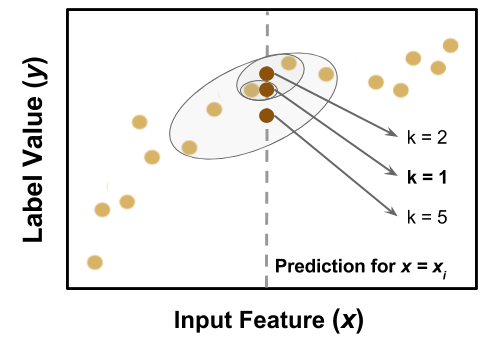
\includegraphics[height=0.5\textheight]{./figures/nn-fig.png}
      \caption{Demonstration of the prediction variation of kNN with different values of \textit{k}}
    \end{figure}
  \end{minipage}
\end{frame}

\begin{frame}
  \frametitle{Decision Trees}
  Objective: many! \\%maximize information gain for each split or minimize \\
  %$$Gain(T, X) = Entropy(T) - Entropy (T, X)$$
  Algorithm hyperparameters of note:
  \begin{itemize}
    \item Maximum \# of features
    \item Maximum depth
    \item Criterion: finish me
  \end{itemize}
  \begin{figure}[h!]
    \centering
    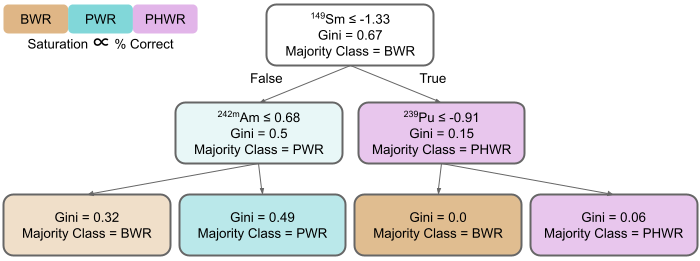
\includegraphics[width=0.7\textwidth]{./figures/dtree.png}
    \caption{Image of a decision tree captured from a simplified example of reactor type prediction}
  \end{figure}
\end{frame}

\begin{frame}
  \frametitle{Maximum Likelihood Calculations}

Likelihood calculated is as follows:
\[L(M|r_{meas}) = \prod_i \frac{1}{\sigma_{i,sim} \sqrt{2\pi}} \exp{\frac{-(r_{i,meas} - r_{i,sim})^2}{2 \sigma_{i,sim}^2}}\]

Whereas the log-likelihood is used in practice:
\[ln(L(M|r_{meas})) = \sum_i ln(\frac{1}{\sigma_{i,sim} \sqrt{2\pi}}) - \frac{(r_{i,meas} - r_{i,sim})^2}{2 \sigma_{i,sim}^2}\]

Approach based on previous work: \cite{mll_method, mll_sensitivity} \\~\\

\end{frame}
